\begin{center}
\textit{Stefano Di Vita, Gauthier Durieux, Jiayin Gu, Zhen Liu, Giuliano Panico, Marc Riembau, Thibaud Vantalon}
\end{center} 

In the previous chapter (cite) it as been shown that assuming the trilinear is the only coupling deviating from its SM value that single Higgs observable can give competitive bound with double Higgs production, see also Refs.~\cite{Gorbahn:2016uoy,Degrassi:2016wml,Bizon:2016wgr,Degrassi:2017ucl,Maltoni:2017ims}, electroweak process where the Higgs trilinear enter at the two loop level have also been studied in \cite{Kribs:2017znd}. Nevertheless, departures of the Higgs self-coupling from its SM prediction signal the existence of new dynamics that, in general, would leave an imprint on other Higgs couplings as well which have a strong impact on the bound as shown by Ref.~\cite{DiVita:2017eyz}. The importance of a global fit is therefore two-fold, namely to assess the robustness of the studies that take into account deformations exclusively in the Higgs trilinear, and to single out the sensitivity on the single-Higgs couplings that is required to minimize the impact of the possible correlations.
	
%{\color{red}In the previous chapter (cite), observables where the Higgs self-coupling enters at leading order, namely double Higgs, as well higher order corrections has been discussed. It as been shown in the literature Refs.~\cite{Gorbahn:2016uoy,Degrassi:2016wml,Bizon:2016wgr,Degrassi:2017ucl} that assuming the trilinear is the only coupling deviating from its SM value that single Higgs observable can give competitive bound with double Higgs production. Nevertheless, departures of the Higgs self-coupling from its SM prediction signal the existence of new dynamics that, in general, would leave an imprint on other Higgs couplings as well which have a strong impact on the bound as shown by Ref.~\cite{DiVita:2017eyz}. The importance of a global fit is therefore two-fold, namely to assess the robustness of the studies that take into account deformations exclusively in the Higgs trilinear, and to single out the sensitivity on the single-Higgs couplings that is required to minimize the impact of the possible correlations.}
	
	
%Departures of the Higgs self-coupling from its SM prediction signal the existence of new dynamics that, in general, would leave an imprint on other Higgs couplings as well. The importance of a global fit is therefore two-fold, namely to assess the robustness of the studies that take into account deformations exclusively in the Higgs trilinear, and to single out the sensitivity on the single-Higgs couplings that is required to minimize the impact of the possible correlations.
\medskip

\begin{figure}
\centering
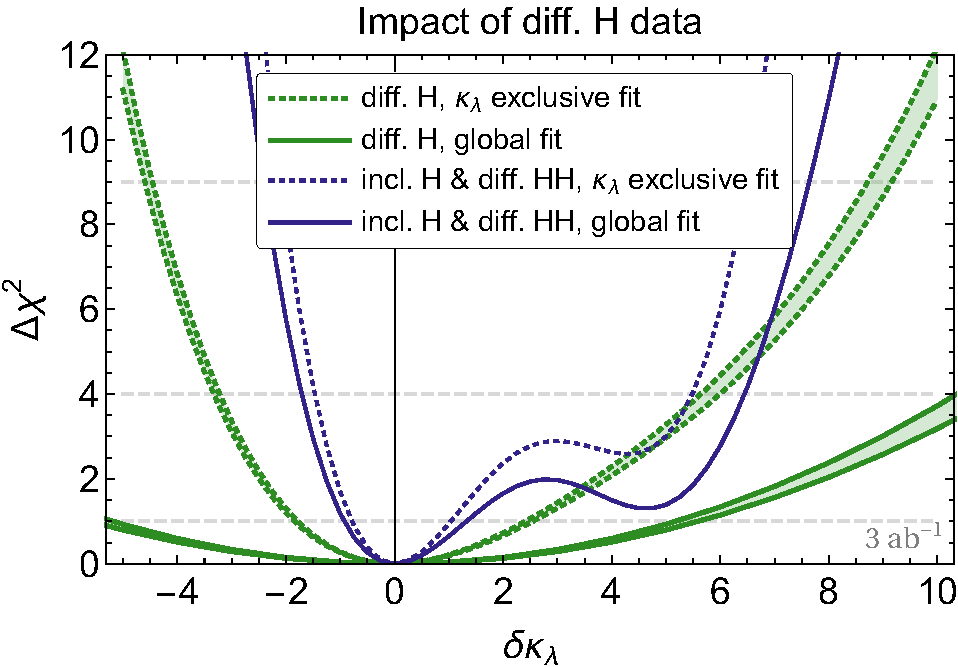
\includegraphics[width=0.45\linewidth]{section3/plots/5leftbisbisbis}\hfill
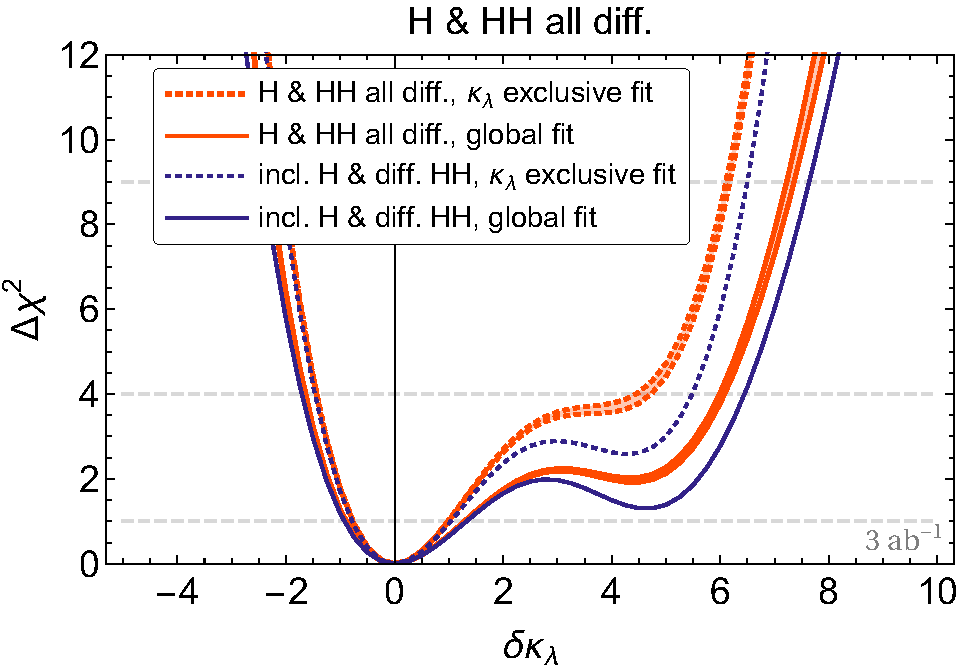
\includegraphics[width=0.45\linewidth]{section3/plots/chi2kl_alldiff_combined}
\caption{$\chi^2$ analysis of the Higgs self-coupling $\delta \kappa_\lambda$ using single- and double-Higgs processes for the HL-LHC at 13\,TeV and 3\,ab$^{-1}$. \textbf{Left:} Comparison of the constraints obtained using differential single-Higgs processes (green), with the ones using differential double-Higgs data together with inclusive single-Higgs measurements (blue). \textbf{Right:} Comparison of the constraints from differential single- and double-Higgs (orange), with those from differential double-Higgs data together with inclusive single-Higgs measurements (blue).}
\label{fig:hllhcchi2}
\end{figure}

To include the effect of the different deformations away from the SM, we use the EFT framework described in Ref.~\cite{DiVita:2017eyz}, where 9 parameters describe the deviations of the single-Higgs couplings. In particular, we consider three\footnote{If other fermionic decay channels can be observed, further parameters can be included, with no effect on the number of degrees of freedom.} parameters for the Yukawa interactions ($\delta y_t,\,\delta y_b,\,\delta y_\tau,$), two for the contact interactions with gluons and photons ($c_{gg}\,,c_{\gamma\gamma}$), rescalings of the SM $hZZ$ and $hWW$ interactions (parametrized by one coefficient, $\delta c_z$, if custodial symmetry is unbroken), and three coefficients ($c_{zz},c_{z\square},c_{z\gamma}$) parametrizing interactions of the Higgs with the electroweak bosons that have non-SM tensor structures. Note that two combinations of the last three parameters are constrained by diboson data, showing an interesting interplay between the gauge and the Higgs sectors. A global fit on the Higgs self-coupling, parametrized by $\delta\kappa_\lambda$ (which is zero in the SM) using only inclusive single Higgs observables, and taking into account the additional 9 EFT deviations described above, suffers from a flat direction. To lift it, it is necessary to include data from differential measurements of those processes, since the single-Higgs deformations and $\delta\kappa_\lambda$ tend to affect the distributions in complementary ways.
\medskip

The global fit for the HL-LHC is summarized in Fig.~\ref{fig:hllhcchi2}. In the left plot, we show in green the $\Delta\chi^2$ including only single-Higgs data, both in an exclusive study (dotted), and after profiling over all the other parameters (solid). The width of the lines corresponds to different assumptions on the extrapolation of the projected experimental sensitivities on the inclusive signal strenghts, to differential ones. We can see that, in a global fit, the constraint on the trilinear is worsened due to correlations (mainly with the top yukawa $\delta y_t$ and the contact interaction with gluons $c_{gg}$, and, to a lesser degree, between $\delta y_b$ and $\delta c_z$ \textbf{refer to fig4 if we include it}). The fit to differential double-Higgs data and inclusive single-Higgs measurements, taken from the study in Ref.~\cite{Azatov:2015oxa}, is depicted in blue. In the right plot we can see that, while double-Higgs is clearly driving the bound, differential single-Higgs data is nonetheless relevant as it can help lift the degenerate minima around $\delta \kappa_\lambda\sim 5$.
\medskip


\begin{figure}
	\centering
	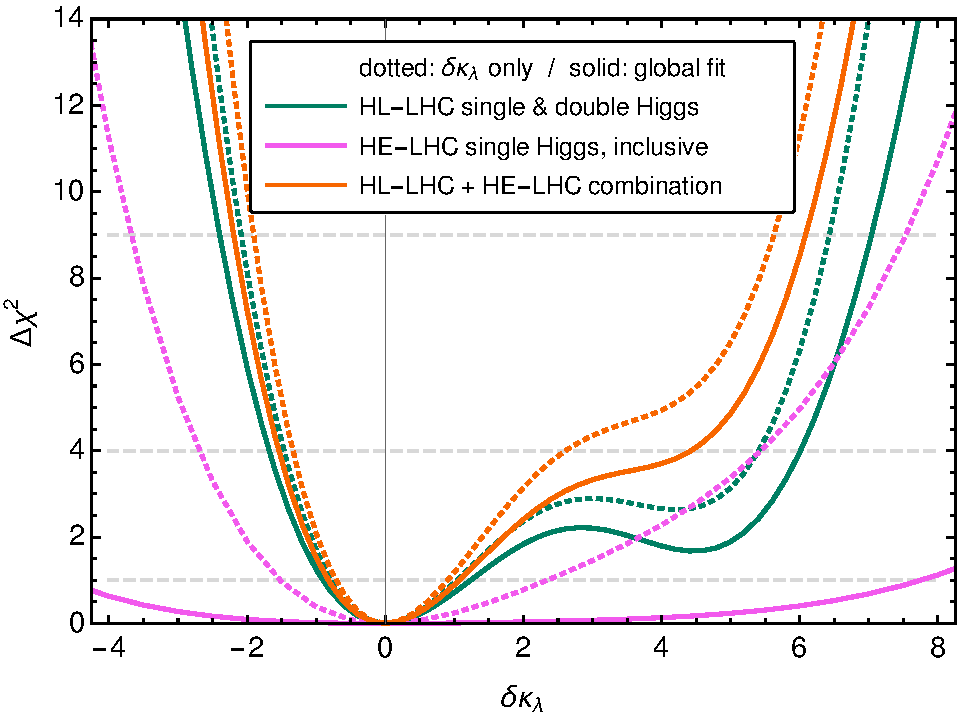
\includegraphics[width=0.45\linewidth]{section3/plots/helhcinc}\hfill
	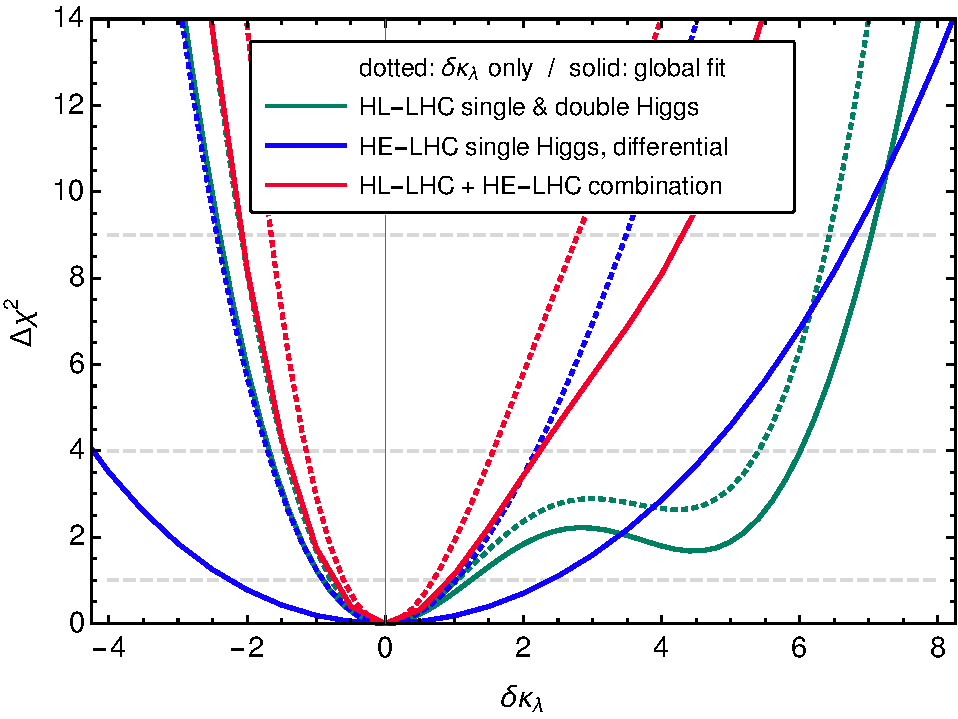
\includegraphics[width=0.45\linewidth]{section3/plots/helhcdiff}
	\caption{$\chi^2$ analysis of the Higgs self-coupling $\delta \kappa_\lambda$ using single-Higgs processes for the HE-LHC at 27\,TeV and 15\,ab$^{-1}$. \textbf{Left:} Comparison of the constraints using inclusive single-Higgs processes at HE-HLC (pink) with the global fit of HL-LHC (green) and its combination (Orange). \textbf{Right:} Comparison of the constraints using differential single-Higgs processes at HE-HLC (blue) with the global fit of HL-LHC (green) and its combination (red).}
	\label{fig:helhcchi2}
\end{figure}	


We now discuss projections for the HE-LHC at 27\,TeV with 15\,ab$^{-1}$ of integrated luminosity. For the uncertainties we perform a simple extrapolation where the theory and systematic uncertainties are kept the same as in the HL-LHC projections, while the statistical uncertainty is rescaled accordingly \cite{Goncalves:2018qas}. We show the results in Fig.~\ref{fig:helhcchi2}. In the left plot, in pink, we present the $\chi^2$ analysis using the projections for the single-Higgs channels at HE-LHC at the inclusive level. Inclusive measurements are able to lift the flat direction due to the measurement of the $th+j$ production and the $z\gamma$ decay. The combination with the full HL-LHC analysis closes the flat direction and the second minimum can be excluded at $\sim 95\%$\,CL. In the right plot the fit using differential observables in single-Higgs production at HE-LHC is shown in blue. The differential information is enough to lift the flat directions and the single-Higgs data is more constraining than the full HL-LHC combination, even in the global fit. Combination with HL-LHC gives a constraint of about $|\delta \kappa_\lambda |\lesssim  2$ at 95\%\,CL. Moreover, the combination (in red) reduces the impact of the correlations.
\medskip

Since it is expected that the theory and systematic uncertainties will change over time, in Fig.~\ref{fig:helhcrescaling} we explore how our findings are affected if both uncertainties are rescaled by a common factor. Getting more than a factor two improvement on those uncertainties, which is a rather reasonable benchmark, does not significantly improve the constraints, and we conclude that the precision is limited by statistics.	
	
\begin{figure}[h]
\centering
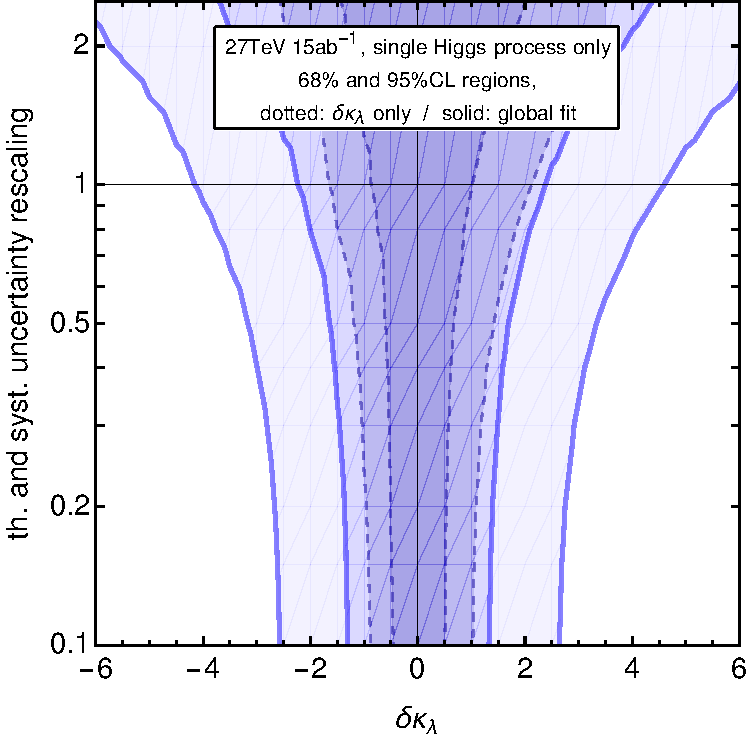
\includegraphics[width=0.4\linewidth]{section3/plots/helhcrescaling}
\caption{$\Delta\chi^2=1$ and $\Delta\chi^2=3.85$ contour regions on the anomalous Higgs self-coupling $\delta \kappa_\lambda$ for the HE-LHC projections, as a function of the common rescaling factor of both the theory and systematic uncertainties with respect to the HL-LHC projections. The dashed lines indicate the constraints for an exclusive fit to $\delta\kappa_\lambda$, while the solid lines indicate the constraints after profiling over the remaining parameters.}
\label{fig:helhcrescaling}
\end{figure}